This chapter introduces and explains the fundamentals to understand the rest of the work presented in this disseration.

\section{Fundamentals on \acl*{SLAM} (\acs*{SLAM})}

From the beginning of civilization, mapping the surroundings has been a key concept for navigating the environment. In essence we faced the same problem as our ancestors: How do we map the environment and know our location within it? \acs*{SLAM} is the challenge of mapping the local environment of a moving entity (e.g. robot) and updating the map continuously as the entity moves through space. This is a massive problem to tackle on and of extreme importance to achieve robot autonomy in moving robots. Even tho we could tecnically divide the problem in two, one being mapping and the other localization, it is not pratical in the real world. Unless the entity has a fixed position, the mapping of an environment will always need some localization information.



A common way to solve this problem is to use a Kalman filter.

\subsection{Kalman Filter}
The Kalman filter is a linear iterative process, as shown in Fig. \ref*{fig: flowchart kalman}, that uses consecutive data input to quickly converge to the true value. Each iteration involves computing three values: the Kalman gain, the current estimate, and its uncertainty. The Kalman gain uses the previous uncertainty and the error in data. The estimate of the current iteration is computed with the new data input and the previous estimation, where the weight of each component is decided by the kalman gain. Once the current estimate has been calculated, the new uncertainty of the estimate is computed with the current estimate and kalman gain.

\begin{figure}[H]
    \centering
    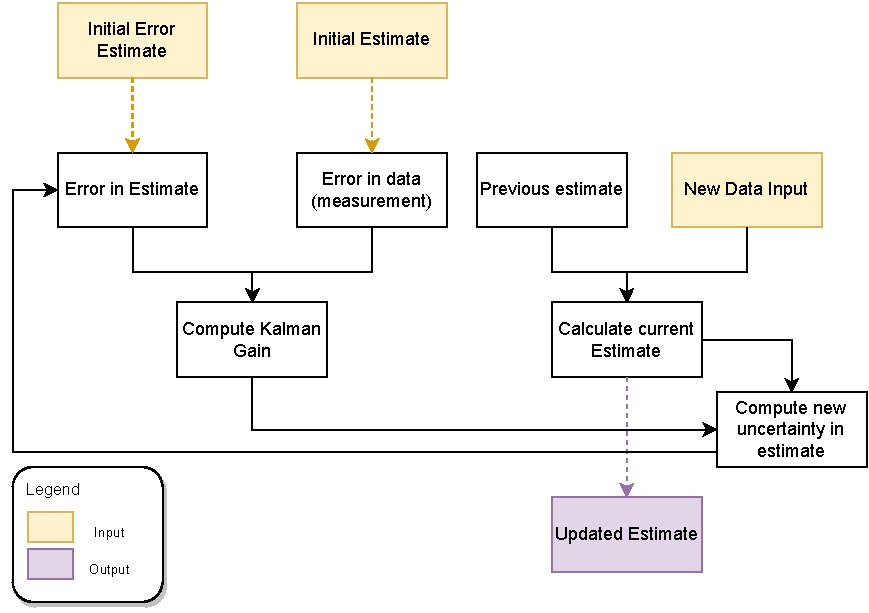
\includegraphics[width=0.7\linewidth]{images/background/Kalman-diagram.pdf}
    \caption{Simple flowchart of the Kalman Filter. \textcolor{red}{ADD REFERENCE}}
    \label{fig: flowchart kalman}
\end{figure}

\subsubsection{\acl{EKF}}

In real world it is uncommon to have a global linear system and due to it's linearity, the Kalman Filter won't work well in non-linear scenarious. A simple way to solve this is to make the global nonlinear function, locally linear, using a first order Taylor Expansion to do the aproximation. This is what the method the \acl{EKF} \acs*{EKF} deploy.

\subsubsection*{\acl*{UKF}}



 A more accurate way to solve the problem is to use a \acl*{UKF} (\acs*{UKF}).


\subsection{Loop Closure}

\subsection{Moving Objects}

\section{\acs{ROS}}

An effective robotics project cannot be achieved by just having sensors and physical components; rather, one must have a clever communication system between sensors and processes. Although such complex systems can be built from scratch, it is not worthwhile when software like \acs*{ROS} is available.

Although the name \acl*{ROS} suggests that ROS is an operating system, this is not the case.  In a way, \acs*{ROS} is both middleware and a framework. The system provides a communication channel where messages can be easily subscribed, published and distributed, allowing quick integration between systems and components. Moreover, it provides features such as debugging, visualization, testing, logging, and configuration right out of the box. Additionally, ROS includes a number of useful packages for essential areas relevant to robotics such as movement, perception, and manipulation. The ROS community is also constantly evolving with the most recent developments in robotics, so libraries are always being added to ROS. In robotics, it is considered the standard platform for developing complex projects.